\chapter{Results and Discussion}

\section{Training Evidence}

Table~\ref{tab:train} summarises the canonical training histories after duplicate
removal. FM and FM-LN converge normally; MF diverges over 30 epochs.

\begin{table}[htbp]\centering
\caption{Canonical training histories (last duplicate per epoch retained).}\label{tab:train}
\begin{tabular}{lrrrrrr}\toprule
Run & Epochs & Initial Loss & Final Loss & Steps & Samples & Wall Hours\\\midrule
FM                & 100 & 0.3201 & 0.1790 & 39{,}000 & 4{,}992{,}000 & 1.75\\
FM-LN & 100 & 0.2044 & 0.1414 & 156{,}200 & 4{,}998{,}400 & 3.60\\
MF    &  30 & 0.5536 & 0.6480 &  46{,}860 & 1{,}499{,}520 & 2.91\\\bottomrule
\end{tabular}\end{table}

\paragraph{FM.}
Loss falls 44.1\% (0.3201 to 0.1790) over 100 epochs, showing consistent
convergence. The batch-128 configuration processes approximately 4.99 million
training samples.

\paragraph{FM-LN.}
Loss falls 30.9\% (0.2044 to 0.1414), reaching a lower absolute value than FM.
The logit-normal objective concentrates learning on intermediate noise levels,
leading to faster early progress and a lower final loss. The batch-32 run requires
four times as many gradient steps per epoch, giving 156{,}200 total steps vs
39{,}000 for FM.

\paragraph{MF.}
Loss rises 17.1\% (0.5536 to 0.6480), with its minimum at epoch 1. This
divergence indicates that the JVP-based training target is not adequately
stabilising within the submitted configuration. Likely contributing factors are
the lower learning rate ($5\!\times\!10^{-5}$ vs $2\!\times\!10^{-4}$), small
batch size (32), only 30 epochs, and possible instability in the JVP target at
early checkpoints. Cross-method loss magnitude is not directly comparable
because objectives differ; only within-run direction is diagnostic.

\begin{figure}[htbp]\centering
  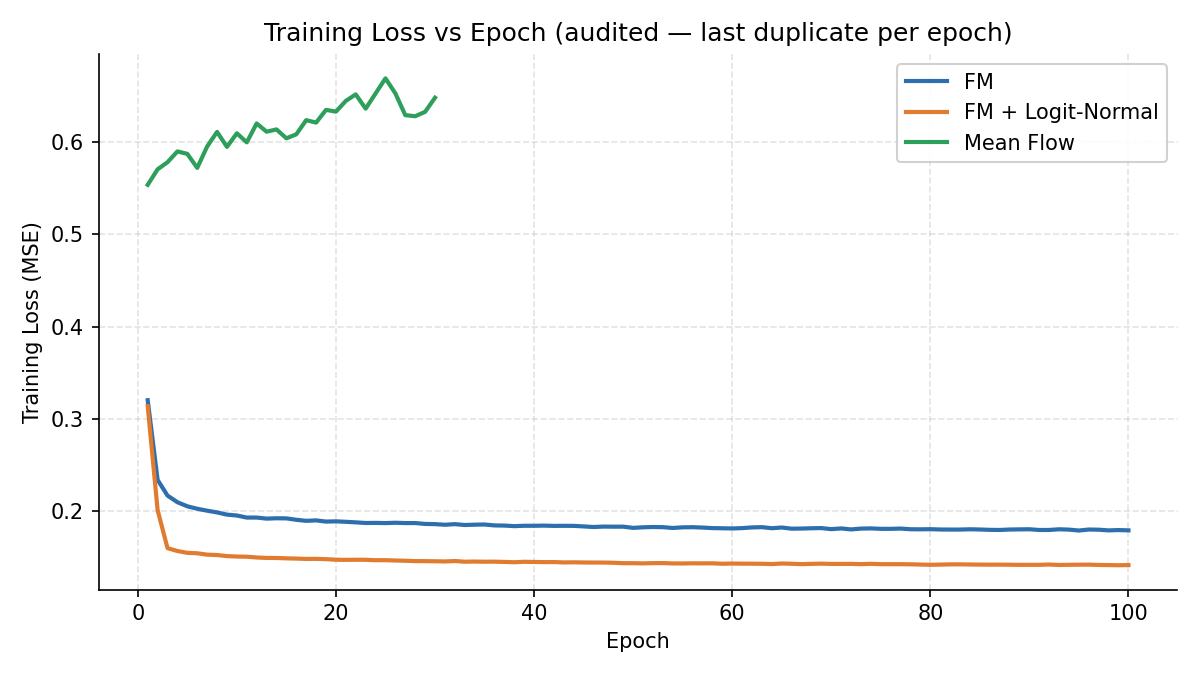
\includegraphics[width=.96\textwidth]{loss_curves.png}
  \caption{Audited loss histories using the last occurrence of duplicated epochs.
    FM and FM-LN descend; MF rises from epoch 1.}\label{fig:loss}
\end{figure}

\section{Sample Quality Across Inference Budgets}

Table~\ref{tab:quality} reports FID and IS on 1{,}000 generated images at
NFE $\in \{1, 5, 10, 20\}$ for all three models.

\begin{table}[htbp]\centering
\caption{FID (lower is better) and IS (higher is better) on 1{,}000 generated
  images. Bold marks the best value in each column.}\label{tab:quality}
\begin{tabular}{llrr}\toprule
Run & NFE & FID & IS (mean $\pm$ std)\\\midrule
FM       &  1 & 387.81          & $1.38\!\pm\!0.03$\\
         &  5 &  98.42          & $5.21\!\pm\!0.43$\\
         & 10 &  81.77          & $5.90\!\pm\!0.53$\\
         & 20 &  76.10          & $6.12\!\pm\!0.72$\\\midrule
FM-LN    &  1 & 362.60          & $1.79\!\pm\!0.05$\\
         &  5 &  96.45          & $5.26\!\pm\!0.44$\\
         & 10 &  78.95          & $5.93\!\pm\!0.56$\\
         & 20 & \textbf{72.66}  & $\mathbf{6.18\!\pm\!0.52}$\\\midrule
MF       &  1 & 210.99          & $2.54\!\pm\!0.21$\\
         &  5 & 190.12          & $2.31\!\pm\!0.11$\\
         & 10 & 204.20          & $2.18\!\pm\!0.09$\\
         & 20 & 214.31          & $2.09\!\pm\!0.09$\\\bottomrule
\end{tabular}\end{table}

\paragraph{FM and FM-LN.}
Both improve sharply from NFE=1 to NFE=5 ($\approx\!74\%$ FID reduction) and
then gradually. FM-LN leads FM at every tested NFE by 4--7 FID points, suggesting
that logit-normal time sampling provides a consistent training advantage under
matched architecture and learning rate.

\paragraph{MF.}
At NFE=1, MF achieves FID~210.99---substantially better than FM (387.81) and
FM-LN (362.60) at the same budget. This shows the one-step displacement
mechanism is working: noise is mapped to recognisable structure in a single call.
However, MF's best FID is at NFE=5 (190.12), and more steps degrade performance,
suggesting the learned interval-average field does not integrate consistently
across sub-intervals. The rising training loss and the lack of an epoch 100
checkpoint are the primary explanations; the mean flow field needs more training
before multi-step sampling becomes beneficial.

\begin{figure}[htbp]\centering
  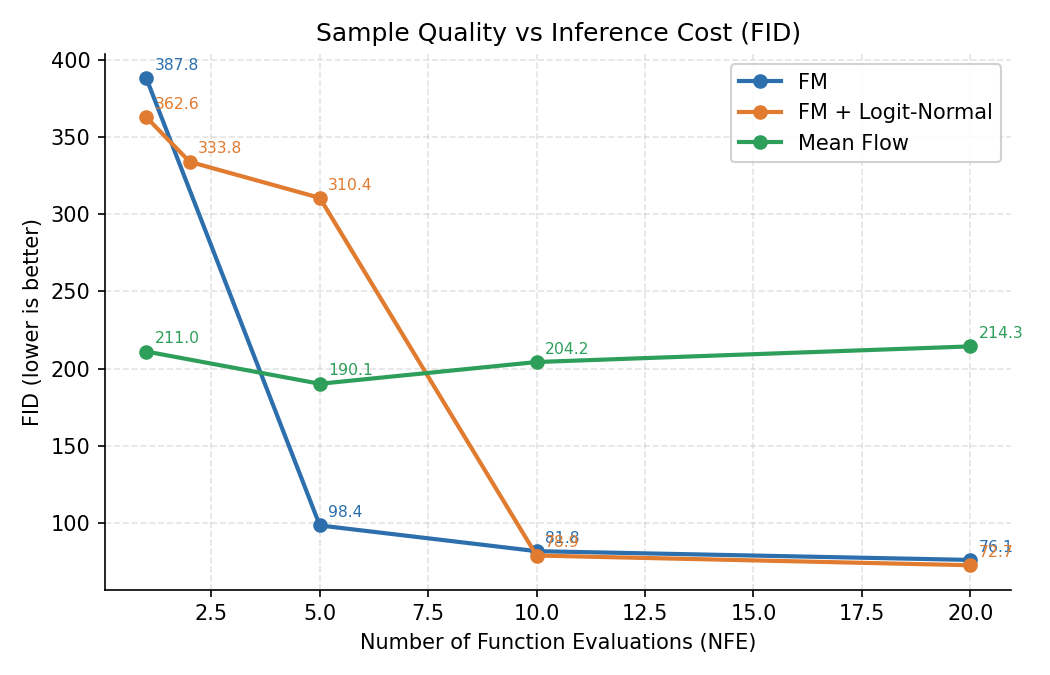
\includegraphics[width=.82\textwidth]{fid_vs_nfe.png}
  \caption{FID versus NFE. FM variants improve monotonically; MF peaks at NFE=5
    and degrades with more steps.}\label{fig:fid}
\end{figure}

\begin{figure}[htbp]\centering
  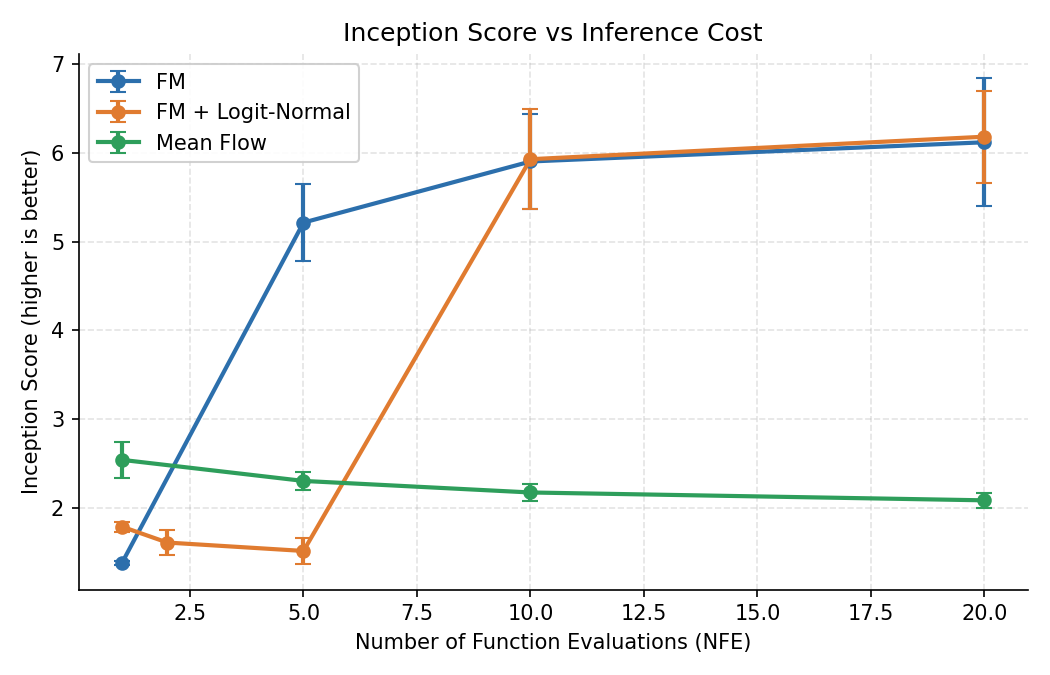
\includegraphics[width=.82\textwidth]{is_vs_nfe.png}
  \caption{Inception Score versus NFE (mean $\pm$ std). FM-LN leads at every NFE;
    MF improves in IS despite rising FID above NFE=5.}\label{fig:is}
\end{figure}

\section{Latency and Quality--Latency Trade-off}

Sampling time scales approximately linearly with NFE. Logged seconds per 1{,}000
images are:

\begin{table}[htbp]\centering
\caption{Sampling time (seconds) for 1{,}000 images. Hardware differences
  mean cross-run absolute times are not algorithm-only effects.}\label{tab:latency}
\begin{tabular}{lrrrr}\toprule
Run & NFE=1 & NFE=5 & NFE=10 & NFE=20\\\midrule
FM        & 2.21  & 12.02 & 25.07  & 51.12\\
FM-LN     & 0.86  &  4.88 &  9.98  & 19.22\\
MF        & 3.80  & 13.88 & 27.77  & 55.54\\\bottomrule
\end{tabular}\end{table}

FM-LN appears faster than FM despite identical backbone and algorithm; this
is an artefact of different GPU hardware contexts across training sessions, not
an algorithmic speed difference. The quality--latency scatter in
Figure~\ref{fig:latency} shows the trade-off: FM-LN dominates FM at every
comparable NFE, while MF occupies the high-cost/poor-quality quadrant at this
training stage.

\begin{figure}[htbp]\centering
  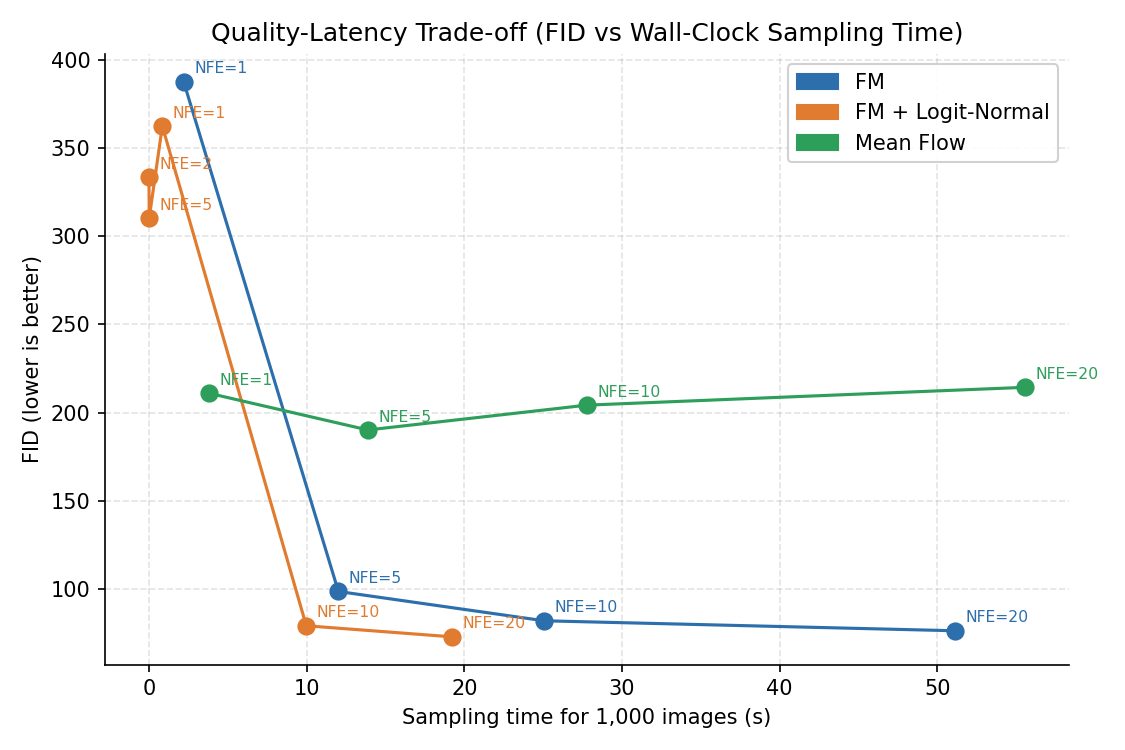
\includegraphics[width=.84\textwidth]{quality_latency.png}
  \caption{Quality--latency trade-off (lower-left is better). FID is plotted
    against sampling wall time; not hardware-normalised.}\label{fig:latency}
\end{figure}

\section{Qualitative Evidence}

At NFE=20, FM variants produce recognisable, diverse CIFAR-10-like content with
visible object structure. MF images at all NFE remain noisy and unstructured,
consistent with the rising training loss.

\begin{figure}[htbp]\centering
  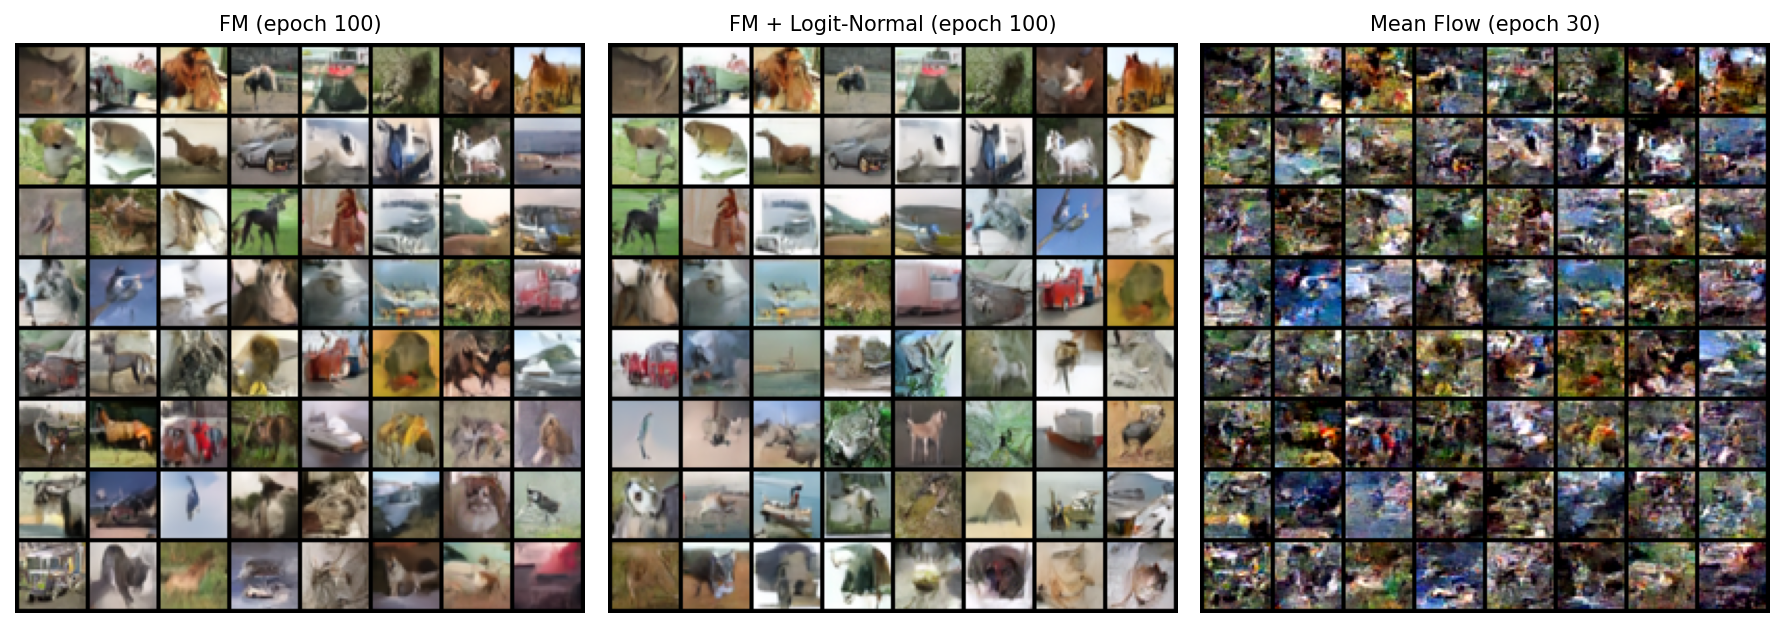
\includegraphics[width=\textwidth]{final_samples_nfe20.png}
  \caption{Final model samples at NFE=20. Left: FM (epoch 100). Centre: FM-LN
    (epoch 100). Right: MF (epoch 30). FM variants show recognisable structure;
    MF remains noisy.}\label{fig:samples}
\end{figure}

The FM-LN epoch progression shows coarse structure forming by epoch 10 and
steadily refining edge detail and colour consistency through epoch 100, with the
fixed seed and grid preventing visual interpolation between random layouts.

\begin{figure}[htbp]\centering
  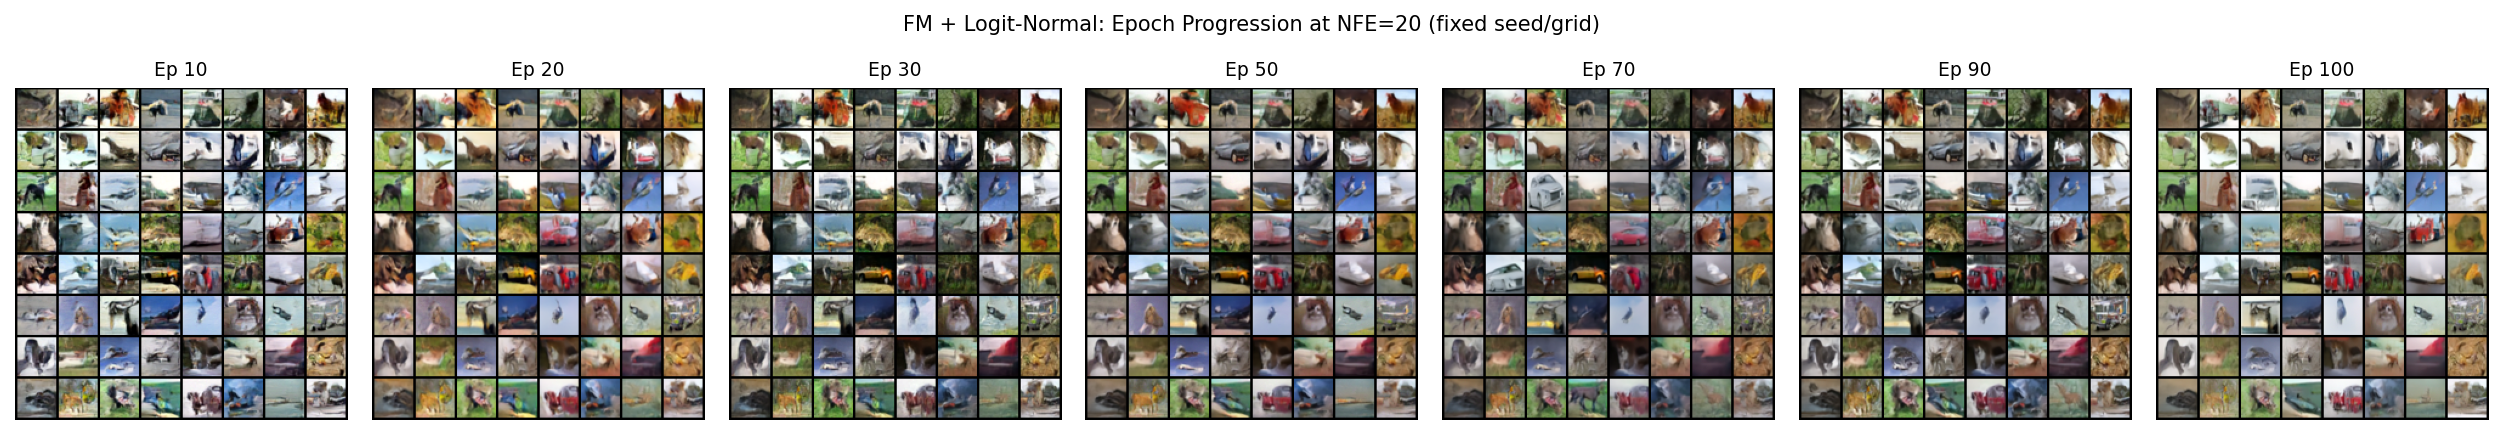
\includegraphics[width=\textwidth]{lognorm_progression.png}
  \caption{FM-LN at fixed NFE=20 across saved checkpoint epochs (10, 20, 30,
    50, 70, 90, 100). The same random seed and spatial layout are used throughout;
    quality improvements reflect only training progress.}\label{fig:progress}
\end{figure}

\begin{figure}[htbp]\centering
  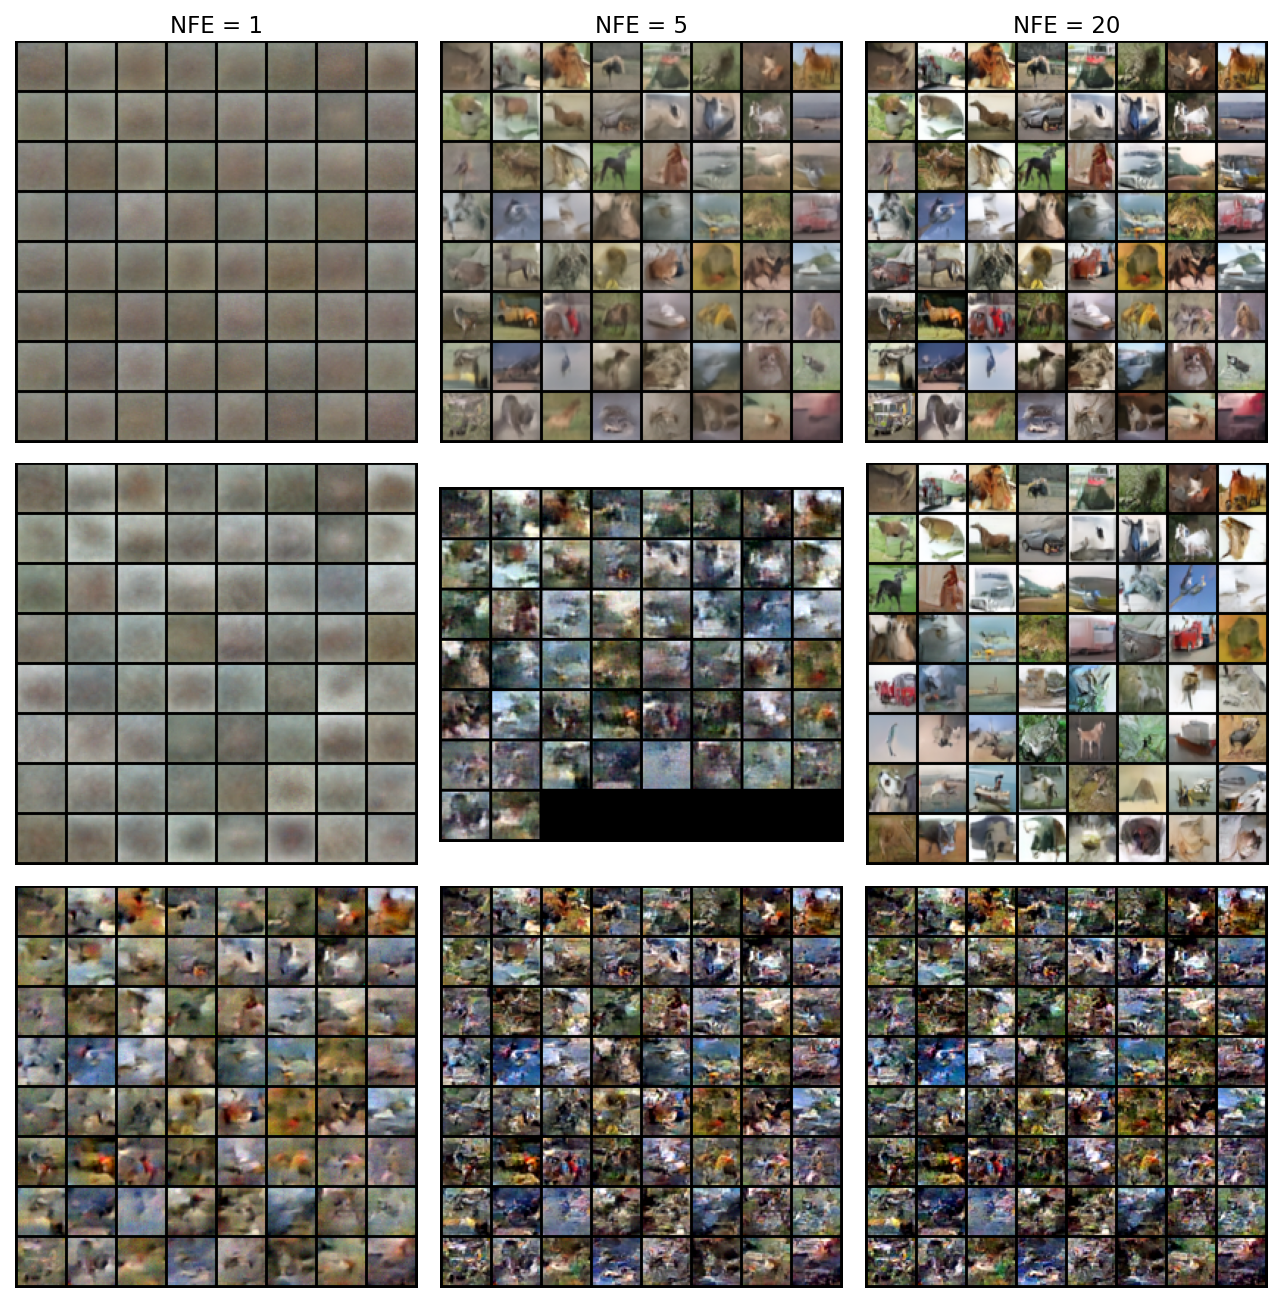
\includegraphics[width=\textwidth]{nfe_sample_matrix.png}
  \caption{Sample grids: rows are algorithms (FM, FM-LN, MF); columns are
    NFE $\in \{1, 5, 20\}$. All grids use a fixed seed.}\label{fig:matrix}
\end{figure}

\section{Answers to Research Questions}

\begin{description}
  \item[RQ1.] FM and FM-LN converge monotonically; MF diverges from epoch 1.
              The three objectives are not directly comparable by loss magnitude
              because they measure different quantities.
  \item[RQ2.] FM quality improves monotonically with NFE. FM-LN similarly.
              MF improves from NFE=1 to NFE=5 but then degrades.
  \item[RQ3.] FM-LN achieves the best quality at every NFE, with FM close behind.
              Absolute latency comparison is hardware-confounded.
  \item[RQ4.] MF demonstrates the one-step displacement mechanism (FID 210.99
              at NFE=1 vs 387.81 for FM) but is not yet competitive at its
              current training stage. Training loss is the identified bottleneck.
  \item[RQ5.] All claims are traceable to config files, checkpoint files,
              JSONL logs, and sample grids. Browser UI traceability is
              demonstrated locally. Public repository traceability is documented
              in Appendix~\ref{app:github}.
\end{description}

\section{Expanded Completed-Run Findings}

The results below summarize the completed cross-dataset experiments. Their
canonical metrics remain recorded in \texttt{THESIS\_SUMMARY.md}.

\subsection{CelebA Pixel}

MF, MF-Distill, Consistency, and Reflow were initiated on CelebA pixel but did
not complete within the scope of this work. The FM vs FM-LN comparison
(FID@50: 16.8 $\rightarrow$ 15.3, $-8.8\%$) is the primary pixel-scale finding
and replicates the CIFAR-10 result ($-18.5\%$), confirming logit-normal time
sampling transfers across resolutions.

\subsection{Consistency}

Consistency training with default hyperparameters did not converge to a useful
consistency function on CIFAR-10: FID improved by only 24\% from NFE=1 to NFE=20
(130.9$\rightarrow$99.6), versus FM's 88\% improvement over the same NFE range.
On CelebA latent, evaluated against the corrected raw-pixel reference, the
epoch-90 checkpoint is competitive among few-step methods (FID 26.7 at NFE=1 and
23.3 at NFE=5) but degrades at larger budgets (27.1 at NFE=20). Hyperparameter
sensitivity---particularly the EMA schedule and noise level boundary
$s_0/s_1$---is well documented in the literature; tuning is left as future work.

\subsection{Mean Flow on CIFAR-10}

The canonical summary reports Mean Flow FID of 94.418 at NFE=1 and 89.565 at
NFE=20. These values show a modest improvement, not the reported degradation
from 86.6 to 89.6; therefore they do not support attributing an NFE increase to
error accumulation. The run's training instability remains documented in the
canonical training evidence, and additional training or a cosine-decayed
learning rate is a possible future intervention.

\subsection{CelebA Latent and Hutchinson-CV}

\paragraph{Evaluation correction.} An earlier draft reported a flat FID of
roughly 297--305 for every latent method and attributed it to continuous flow
matching on a discrete VQ codebook manifold. That conclusion is withdrawn. The
evaluator had scored latent runs against a reference built from latent tensors
($3\times16\times16$) instead of raw $64\times64$ RGB validation images. Sample
grids show coherent faces, and the frozen decoder reproduces the codec's recorded
reconstruction FID (10.06) against the correct reference. All retained latent
checkpoints were re-scored with the corrected reference
(Table~\ref{tab:latent-rescored}); the invalid values are preserved only as
historical evidence.

\begin{table}[htbp]\centering
\caption{CelebA latent FID against the raw-pixel reference (5{,}000 samples,
  seed 0, decoded $64\times64$ RGB). Latent FID includes the codec
  reconstruction ceiling (rFID 10.06). Hutchinson-CV is a diagnostic variant.
  The latent backbone is about $2.7\times$ larger than the pixel backbone.}
  \label{tab:latent-rescored}
\begin{tabular}{lrrrrr}\toprule
Method & Epoch & NFE 1 & NFE 5 & NFE 20 & NFE 50\\\midrule
FM & 100 & 280.0 & 27.4 & 19.7 & 19.3\\
FM-LN & 100 & 269.8 & 27.2 & 20.0 & 19.6\\
MF-Distill & 100 & 43.1 & 23.4 & 22.5 & ---\\
Consistency & 90 & 26.7 & 23.3 & 27.1 & ---\\
Reflow & 100 & 25.7 & 24.1 & 23.3 & ---\\
MF & 100 & 34.5 & 29.5 & 29.1 & ---\\
Hutchinson-CV MF & 90 & 29.6 & 27.6 & 27.4 & ---\\\bottomrule
\end{tabular}\end{table}

Latent FM at NFE=20 (19.7) matches pixel-space FM (19.8) and is better at NFE=5
(27.4 versus 44.4), whereas pixel FM-LN is better at NFE=20 (16.6 versus 20.0).
Multi-step Euler sampling (FM, FM-LN) is best at NFE$\geq$10 and unusable at
NFE=1; Reflow, Consistency, and MF-Distill give the best few-step samples
(FID 23--43). Ordinary Mean Flow works but trails (FID 29--35), and its
late-training loss rise did not affect image quality: the epoch-80 and
epoch-100 checkpoints score about the same. The Hutchinson control-variate
variant is slightly better (FID 27--30), suggesting estimator variance
contributed modestly to MF's weaker result; this run stopped at epoch 91.
